\documentclass{article}
\usepackage{packages}

\title{Коллоквиум по Математическому анализу-2, семестр 2}
\author{Виноградова Дарья, Залялов Александр, Миронов Алексей, Стрельцов Артём, Шамаилов Гершон}
\date{}

\begin{document}

	\maketitle

	\tableofcontents

    \clearpage
    
    \section*{Реклама}
    \href{https://t.me/applied_memes}{@applied\_memes}\par
    \href{https://t.me/fcs_channels}{@fcs\_channels}

	\setcounter{section}{0}
	
	\section{Пространство кусочно-непрерывных функций на отрезке как пример евклидова пространства. Неравенство Коши-Буняковского на этом пространстве (б.д.). Ортогональные и ортонормированные системы в евклидовом пространстве. Главный пример: $C([-\pi; \pi])$}
	
	Напомним, что евклидово пространство - это векторное пространство над полем вещественных чисел со скалярным произведением.
	
	\textit{Свойства скалярного произведения:}
	
	1. $\langle u, v \rangle=\langle v, u\rangle$
	
	2. $\langle \lambda_1 u_1 + \lambda_2 u_2, v\rangle=\lambda_1 \langle u_1, v\rangle+\lambda_2 \langle u_1, v \rangle$
	
	3. $\langle v,v \rangle \ge 0$
	
	3'. $\langle v,v \rangle = 0 \Rightarrow v=0$\\
	
	Рассмотрим векторное пространство $V=\hat C([a; b])$ - множество кусочно-непрерывных функций на $[a; b]$ (имеющих конечное число точек разрыва первого рода), обладающих также следующим свойством:
	
	$f(c)=\frac{1}{2}(\lim\limits_{x \rightarrow c-0} f(x) + \lim\limits_{x \rightarrow c+0} f(x))$
	
	 Определим на $\hat C$ скалярное произведение $\langle f, g \rangle =\int\limits_a^b f(x)g(x)dx$ и проверим свойства, чтобы показать его корректность.
	
	1-3 очевидны. 3' сначала рассмотрим для непрерывной на отрезке функции. 
	От противного: пусть на отрезке существует какая-то точка $c$, в которой функция принимает ненулевое значение. Тогда $f^2(c) > 0$. В силу непрерывности есть такая окрестность $(c-\delta; c+\delta)$, в которой $f^2(x) \ge \epsilon > 0$.
	
	$\int\limits_a^b f^2(x) \ge \int\limits_{c-\delta}^{c+\delta} f^2(x) \ge 2\delta\epsilon > 0$
	
	Для $\hat C$ отрезок разваливается на конечное число отрезков непрерывности, применим к ним предыдущее.
	
	\begin{theorem} (неравенство Коши-Буняковского) $\langle f, g \rangle^2 \le \langle f, f \rangle \cdot \langle g, g \rangle$ \end{theorem}
	
	Для нашего пространства оно имеет вид 
	
	$(\int\limits_a^b f(x)g(x)dx)^2 \le \int\limits_a^b f^2(x)dx \int\limits_a^b g^2(x)dx$
	
	\begin{definition}
		Множество элементов  ${\psi_i} \in V$ называется \textit{ортогональной} системой, если для любой пары $\langle \psi_i, \psi_j\rangle=0$. Если при этом $\| \psi_i \|=1$ $\forall i$, то система \textit{отронормирована}.
	\end{definition}

	В $C([-\pi; \pi])$ следующая система является ортонормированной:
	
	$\{{\frac{1}{\sqrt{2\pi}}, \frac{1}{\sqrt{\pi}}\cos x, \frac{1}{\sqrt{\pi}}\sin x, \frac{1}{\sqrt{\pi}}\cos {2x}, \cdots}\}$\\
	
	Проверим норму на примере $\cos$:
	
	$\| \frac{1}{\sqrt{\pi}}\cos {kx}\|= \frac{1}{\sqrt{\pi}}
	 \sqrt{\int\limits_{-\pi}^{\pi} \cos^2 (kx) dx}=
	 \frac{1}{\sqrt{2\pi}} \sqrt{\int\limits_{-\pi}^{\pi} \cos(2kx) + 1}=\frac{1}{\sqrt{2\pi}} \sqrt{2\pi}=1$
	
	Любая функция с $\cos$ ортогональна любой с $\sin$ в силу нечетности. Проверим ортогональность двух функций с $\cos$:
	
	$\langle \frac{1}{\sqrt{\pi}} \cos(kx), \frac{1}{\sqrt{\pi}}\cos(lx) \rangle=\frac{1}{\pi}\int\limits_{-\pi}^{\pi}\cos(kx) \cos(lx) dx=\frac{1}{2\pi}\int\limits_{-\pi}^{\pi}(\cos((k+l)x)+\cos((k-l)x)) dx=0$
	
	Остальное оставим в качестве упражнения для пытливого читателя.
	
	\section{Задача о наилучшем приближении элемента евклидова пространства элементом конечномерного пространства (б.д.). Ряд Фурье по произвольной ортонормированной системе. Ряд Фурье по тригонометрической системе.}
	
	Пусть имеется ортонормированная система $\{{\psi_i}\}$ в векторном пространстве $V$. Хотим найти наилучшее приближение элемента $f$ этого пространства вида $\sum c_k \psi_k$ (т.е. $\|f-\sum c_k \psi_k\| \rightarrow min$). Утверждается, что $c_k=\langle f, \psi_k\rangle$.
	
	 \begin{definition}
	 	\textit{Ряд Фурье по произвольной ортонормированной системе $\{{\psi_i}\}$} - это сумма вида $\sum c_k \psi_k$
	 \end{definition}
 
	 \begin{definition}
	 	\textit{Ряд Фурье по тригонометрической системе} - это сумма вида $\frac{f_0}{\sqrt{2\pi}} +\sum \frac{f_k}{\sqrt{\pi}}cos(kx) + \frac{\hat f_k}{\sqrt{\pi}}sin(kx)$, где $f_0=\frac{1}{\sqrt{2\pi}}\int\limits_{-\pi}^{\pi} f(x) dx$, $f_k=\frac{1}{\sqrt{\pi}}\int\limits_{-\pi}^{\pi} f(x)cos(kx), \hat f_k=\frac{1}{\sqrt{\pi}}\int\limits_{-\pi}^{\pi} f(x)sin(kx) dx$
	 \end{definition}
 
 	Обычно ряд Фурье записывают как $\frac{a_0}{2} + \sum a_k cos(kx) + b_k sin(kx)$,
 	
 	где $a_0=\frac{1}{\pi}\int\limits_{-\pi}^{\pi} f(x) dx$, $a_k=\frac{1}{\pi}\int\limits_{-\pi}^{\pi} f(x)cos(kx), b_k=\frac{1}{\pi}\int\limits_{-\pi}^{\pi} f(x)sin(kx) dx$
	
	\section{Неравенство Бесселя (идея доказательства). Определения замкнутой и полной ортонормированных систем (ОНС). Тождество Парсеваля для замкнутой ОНС.}
	
	\begin{theorem} 
		(неравенство Бесселя) $\sum_{i=1}^{\infty} \langle f, \psi_i \rangle^2 \le \| f \|^2$, где $f$ - элемент векторного пространства $V$ с ортонормированной системой $\{{\psi_i}\}$. Далее $f_i=\langle f, \psi_i \rangle$
	\end{theorem}
	\begin{proof}
		$0 \le \| f- \sum_{i=1}^{n} \langle f \psi_i \rangle \|^2=\|f\|^2-\sum_{i=1}^{n} \|\langle f, \psi_i \rangle \|^2=\|f\|^2-\sum_{i=1}^{n} f_i ^2$ 
		
		$\sum_{i=1}^{n} f_i^2$ ограничена сверху $\|f\|^2$ $\Rightarrow$  сходится. Переходим к пределу, получаем требуемое. 
	\end{proof}

	\begin{definition}
		Ортонормированная система \textit{замкнута}, если $\forall \epsilon > 0 \; \exists n \in \mathbb{N} \; \exists c1, \cdots, c_n \; \| f-\sum_{i=1}^{n} c_k \psi_k\| < \epsilon$
	\end{definition}

	\begin{definition}
		Ортонормированная система \textit{полна}, если $[\; \forall k \in \mathbb{N} \ \Rightarrow f \perp \psi_k] \Rightarrow f \equiv 0$
	\end{definition}

	\begin{theorem} 
		(тождество Парсеваля) Для замкнутой ортонормированной системы  $\sum_{i=1}^{\infty} f_k^2 = \| f \|^2$ 
	\end{theorem}
	\begin{proof}
		Зафиксируем $\epsilon$.
		Из определения замкнутости $\exists n \in \mathbb{N} \; \exists c1, \cdots, c_n \; \| f-\sum_{i=1}^{n} c_k \psi_k\| < \epsilon$. 
		
		Из неравенства Бесселя $\|f\|^2-\sum_{i=1}^{n} f_i ^2 \le \| f-\sum_{i=1}^{n} c_k \psi_k\|^2 \le \epsilon^2$. 
		
		Тогда для $m \ge n$ и подавно $\|f\|^2-\sum_{i=1}^{m} f_i ^2 \le \| f-\sum_{i=1}^{n} c_k \psi_k\|^2 \le \epsilon^2$
		
		Значит, $\forall \epsilon > 0 \; \exists n \in \mathbb{N} \; \forall m \ge n \; \|f\|^2-\sum_{i=1}^{m} f_i ^2 \le \epsilon^2$, и из этого и следует равенство в пределе.
	\end{proof}
	
	\section{Бывают ли замкнутые ортонормированные системы, но не полные?}
	
	Не бывает. Пусть $\forall i \; f\perp \psi_i$. Значит, $f_i=0$. В силу замкнутости справедливо тождество Парсеваля. то есть $\|f\|^2=\sum_{i=1}^{\infty}f_i=0$
	
	\section{Дайте определение свертки двух функций $f, g: \mathbb{R}^n \to \mathbb{R}$. Докажите, что операция свертки коммутативна. Дайте определение свертки двух $2\pi$-периодических функций $f, g: \mathbb{R} \to \mathbb{R}$.}
	
	\begin{definition}
		\textit{Сверткой} функций $f, g: \mathbb{R}^n \to \mathbb{R}$ называется $(f*g)(t)=\int\limits_{\mathbb{R}^n} f(x)g(t-x)dx$
	\end{definition}

	\begin{theorem} 
		$(f*g) \equiv (g*f)$ 
	\end{theorem}
	\begin{proof}
		Положим $\tau=t-x$.
		
		$\int\limits_{\mathbb{R}^n} f(x)g(t-x)dx =\int\limits_{\mathbb{R}^n} f(t-\tau)g(\tau)d\tau$ - область интегрирования не поменялась, а функция домножилась на модуль якобиана замены. В данном случае он равен $1$.
	\end{proof}
	\begin{definition}
		\textit{Сверткой} $2\pi$-периодических функций $f, g: \mathbb{R} \to \mathbb{R}$ называется $(f*g)(t)=\int\limits_{-\pi}^{\pi} f(x)g(t-x)dx$
	\end{definition}
	
	\section{Дайте определения ядра Дирихле и ядра Фейера. Какой смысл у свертки произвольной периодической функции с этими ядрами? (б.д.)}
	
	\begin{definition}
		\textit{Ядром Дирихле} называется $D_n(t)=\frac{\sin[(n+\frac{1}{2})t]}{2\sin{\frac{t}{2}}}$
	\end{definition}

	Обозначим $S_n(x,f)=\frac{a_0}{2} + \sum_{k=1}^{n} a_k cos(kx) + b_k sin(kx)$, где $f$ - $2\pi$-периодическая и интегрируемая на $[-\pi; \pi]$. 
	
	Тогда справедливо $S_n(x, f)=\frac{1}{\pi}\int\limits_{-\pi}^{\pi}f(x+t)D_n(t) dt$ - то есть свертка с ядром Дирихле дает нам $n$-ю частичную сумму ряда Фурье.

	\begin{definition}
		\textit{Ядром Фейера} называется $\Phi_n(t)=\frac{\sin^2(\frac{tn}{2})}{2\sin^2{\frac{t}{2}}}$
	\end{definition}

	Обозначим $\sigma_n(x,f)=\frac{S_0(x, f)+\cdots+S_{n-1}(x, f)}{n}$ - среднее арифметическое ряда Фурье. 
	
	Для $f$ с теми же свойствами будет верно $\sigma_n(x, f)=\frac{1}{n\pi}\int\limits_{-\pi}^{\pi}f(x+t)\Phi_n(t) dt$
	 
	\section{Сформулируйте (б.д.) теоремы о приближении $2\pi$ периодической функции тригонометрическими многочленами: о сходимости ядра Фурье в точке, и о приближении функции тригонометрическими многочленами в различных функциональных метриках.} 
	
	\begin{theorem} 
		Если $2\pi$-периодическая функция имеет в точке производную слева и справа, то ряд Фурье в ней сходится к среднему арифметическому этих производных.
	\end{theorem}

	Заметим, что в условиях данной теоремы функция может быть разрывной.\\
	
	Еще раз напомним, что $\sigma_n(x,f)=\frac{S_0(x, f)+\cdots+S_{n-1}(x, f)}{n}$
	
	\begin{theorem} 
		Пусть $f$ - непрерывная $2\pi$-периодическая функция. Тогда $\sigma_n \rightarrow f$ на $[-\pi, \pi]$ в смысле метрики $d_{\infty}$
	\end{theorem}

	\begin{theorem} 
		Пусть $f$ - кусочно-непрерывная. Тогда ее можно приблизить тригонометрическим многочленом в смысле метрики $d_2$.
	\end{theorem}



	\usepackage{commath}

\makeatletter
\newcommand*{\toto}[2]{\mathrel{
  \settowidth{\@tempdima}{$\scriptstyle#1$}
  \settowidth{\@tempdimb}{$\scriptstyle#2$}
  \ifdim\@tempdimb>\@tempdima \@tempdima=\@tempdimb\fi
  \mathop{\vcenter{
    \offinterlineskip\ialign{\hbox to\dimexpr\@tempdima+1em{##}\cr
    \rightarrowfill\cr\noalign{\kern.5ex}
    \rightarrowfill\cr}}}\limits^{\!#1}_{\!#2}}}
\makeatother


\title{Билеты 8-13}
\author{}
\date{}
\begin{document}
\maketitle

\setcounter{section}{7}
\section{Сформулируйте (б.д.) лемму Римана. Какова связь между порядком дифференцируемости $2\pi$-периодической функции и асимптотикой ее коэффицинтов Фурье? Ответ поясните.}
\begin{lemma} (Риман).
    Пусть $f$ абсолютно интегрируема на промежутке $(a, b)$. Тогда
    $$
        \lim\limits_{\omega\to\infty}\int_{a}^{b}f(x)\sin(\omega x)dx = 0
    $$
    $$
        \lim\limits_{\omega\to\infty}\int_{a}^{b}f(x)\cos(\omega x)dx = 0
    $$
\end{lemma}

\begin{corollary}
    Если $f$ интегрируемая и $2\pi$-периодическая, то ее коэффициенты $a_n, b_n$ ряда Фурье стремятся к 0ю
\end{corollary}

\begin{corollary}
    Пусть $f$ -- $2\pi$-периодическая и имеет $s - 1$ производную, а $f^{(s - 1)}$ -- кусочно-гладкая. Тогда ряд Фурье для $f^{(s)}$ получается $s$-кратным почленным дифференцированием ряда Фурье для $f$. При этом, $a_n, b_n = \overline{o}\left(\frac{1}{k^s}\right)$ при $k\to\infty$
\end{corollary}
Почему второе следствие верно? Интуитивно: чтобы выполнялась лемма Римама, требуется, чтобы коэффициенты стремились к 0. При дифференцировании $s - 1$ раз у нас столько же раз <<вылезет>> $k$ из косинуса и синуса, поэтому, чтобы все еще выполнялась сходимость к 0, нужно, чтобы $a_n, b_n = \overline{o}\left(\frac{1}{k^s}\right)$.

\section{Дайте определение преобразования Фурье для функции $\mathbb{R}\to\mathbb{C}$, приведите пример вычисления преобразования Фурье. Пусть $f\in L_1(\mathbb{R})$. Сформулируйте основную теорему об образе преобразования Фурье.}
\begin{definition}
    Пусть $f\colon\mathbb{R}\to\mathbb{C}$. Если выражение $$\hat{f}(y) = F[f](y) = v.p.\int_{-\infty}^{+\infty}f(x)e^{ixy}dx$$ определено для всех $y\in\mathbb{R}$, то $\hat{f}\colon\mathbb{R}\to\mathbb{C}$ называется преобразованием Фурье.
\end{definition}

Например, пусть $f(x) = I_{[-1, 1]}(x)$. Тогда
$$
    \hat{f}(y) = \int_{-\infty}^{+\infty}I_{[-1, 1]}(x)e^{ixy}dx = \int_{-1}^{1}e^{ixy}dx = \int_{-1}^{1}\cos(xy)dx + i\int_{-1}^{1}\sin(xy)dx = \frac{\sin(xy)}{y}\Big|_{-1}^{1} = 2\frac{\sin y}{y}
$$

\begin{definition}
    $L_1(\mathbb{R})$ -- пространство функций, абслолютно интегрируемых на $\mathbb{R}$.
\end{definition}

\begin{theorem} (Основная теорема об образе Фурье)
    Если $f\in L_1(\mathbb{R})$, то
    \begin{enumerate}
        \item Функция $\hat{f}$ корректно определена.
        \item Функция $\hat{f}$ непрерывна.
        \item $\lim\limits_{y\to\pm\infty}\hat{f}(y) = 0$
    \end{enumerate}
\end{theorem}

\section{Что вы можете сказать о функции $\hat{f}$, если (1) $f$ четная и вещественнозначная (2) $f$ четная и вещественнозначная.}
\begin{lemma}
    \begin{enumerate}
        \item Если $f$ -- четная, то $F^{-1}[f] = \frac{1}{2\pi}F[f]$
        \item Если $f$ -- нечетная, то $F^{-1}[f] = -\frac{1}{2\pi}F[f]$
    \end{enumerate}
\end{lemma}

\begin{proof}
    \begin{enumerate}
        \item $F[f](y) = \int_{-\infty}^{\infty}f(x)e^{ixy}dx = \int_{-\infty}^{\infty}f(-x)e^{ixy}dx = [\textrm{Замена $x$ на $-x$}] = \int_{-\infty}^{\infty}f(x)e^{-ixy}d(-x) = \int_{\infty}^{-\infty}f(x)e^{-ixy}d(x) = 2\pi F^{-1}[f]$
        \item Доказывается абсолютно аналогично. При замене $x$ на $-x$ просто еще и поменяется знак у интеграла.
    \end{enumerate}
\end{proof}

\section{Дайте определение интеграла Фурье и обратного преобразования Фурье. Сформулируйте и докажите теорему о свертке. Чему равно преобразование Фурье от произведения двух функций?}
\begin{definition}
    Интегралом Фурье от функции $f\colon \mathbb{R}\to\mathbb{C}$ в точке $x$ называется выражение $$\frac{1}{2\pi} v.p.\int_{-\infty}^{\infty}\hat{f}(y)e^{-ixy}dy$$
\end{definition}

\begin{definition}
    Пусть $f$ дифферецируемая функция, тогда преобразование
        $$\hat{f}(y) \to f(x) = \frac{1}{2\pi} v.p.\int_{-\infty}^{\infty}\hat{f}(y)e^{-ixy}dy$$
    называется обратным преобразованием Фурье.
\end{definition}

\begin{theorem} (О свертке)
    Если $f, g\in L_1(\mathbb{R})$, то $F(f\star g) = F[f]\cdot f[g]$.
\end{theorem}
\begin{proof}
    $$
    F[f\star g](y) = \int_{-\infty}^{+\infty}(f - g)(x)e^{ixy}dx = \int_{-\infty}^{+\infty}\left(\int_{-\infty}^{+\infty}f(s)g(x - s)ds\right)e^{ixy}dx
    $$
    Благодаря абсолютной интегрируемости, можем поменять порядки интегрирования, а следовательно, просто в виде кратного:
    $$
    \iint_{\mathbb{R}^2} f(s)g(x - s)e^{ixy}dxds
    =
    \begin{bmatrix}
        u = s \\
        v = x - s \\
        dxds = dudv
    \end{bmatrix}
    =
    \int_{-\infty}^{+\infty} f(u)e^{iuy}du\cdot \int_{-\infty}^{+\infty} g(v)e^{ivy}dv = F[f] \cdot F[g].
    $$
    Аналогично можно доказать для обратного преобразования.
\end{proof}

\begin{corollary}
    $F[f\cdot g] = \frac{1}{2\pi}F[f]\star F[g]$
\end{corollary}

\section{Выведите формулу для производной $\hat{f}(y)$. Какова связь дифференцируемости функции $f(x)$ и асимптотики ее преоразования Фурье $\hat{f}(y)$ при $y\to\infty$}

\begin{statement}
    Пусть $f(x)$ такова, что $f(x)(1 + \abs{x})^k\in L_1(\mathbb{R})$. Тогда $\hat{f} = F[f]$ дифференцируема $k$ раз, причем производные $\hat{f}$ можно вычислить дифференцированием под знаком интеграла.
\end{statement}

\begin{proof}
    Это следует из теорем прошлого семестра (что можно дифференцировать по параметру, в нашем случае по $y$, под знаком интеграла, если есть равномерная сходимость по $x$).
    $$
    F[f](y) = v.p.\int_{-\infty}^{+\infty}f(x)e^{ixy}dx
    $$
    $\forall\; m \le k$ верно
    $$
    \abs{f(x)e^{ixy}(ix)^m} \le \abs{f(x)}(1 + \abs{x})^m
    $$
    В левой части стоит просто продифференцированное $m$ раз подынтегральное выражение в преобразовании Фурье. Неравенство следует из ограниченности $\abs{e^{ixy}\cdot i^m} \le 1$. В правой части стоит функция, интегрируемая на $\mathbb{R}$ (по условию).\\
    При этом левая часть сходится равномерно по $y$. Значит, можем пользоваться теоремой из прошлого семестра:
    $$
        \frac{d^m}{dy^m}\hat{f}(y) = \int_{-\infty}^{+\infty}f(x)e^{ixy}(ix)^mdx
    $$
    Отсюда же получаем формулу:
    $$
    \frac{d^m}{dy^m}F[f](y) = F[(ix)^m f(x)]
    $$
\end{proof}

\begin{statement}
    Пусть $f$ дифференцируема $k$ раз во всех точках, причем $f^{(m)}\in L_1(\mathbb{R})$ при $m = 0, \ldots, k$ и $f^{(m)}(x)\to 0$ при $x\to\infty$ и $m = 0, \ldots, k$, тогда $\hat{f}(y) = \overline{o}\left(\frac{1}{\abs{y}^k}\right)$ при $t\to\infty$
\end{statement}

\begin{proof}
    Запишем $F[f^(k)]$:
    $$
    \int_{-\infty}^{+\infty}f^{(k)}(x)e^{ixy}dx = \int_{-\infty}^{+\infty}e^{ixy}df^(k - 1) = e^{ixy}f^{(k - 1)}(x)\Big|_{-\infty}^{+\infty} - \int_{-\infty}^{+\infty}f^{(k - 1)}(x)\cdot (iy)e^{ixy}dx =
    \begin{bmatrix}
    \textrm{Далее аналогично.} \\
    \textrm{Также пользуемся тем, что }\\
    \lim\limits_{x\to\infty}f^{(m)} = 0\;\;\forall m = 0, \ldots, k
    \end{bmatrix}
    $$
    $$
    =
    \int_{-\infty}^{+\infty}f(x)e^{ixy}(-1)^m (iy)^m dx
    =
    (-iy)^k F[f](y) = (-iy)^k \hat{f}(y)
    $$
    Также мы знаем, что если функция абсолютно интегрируемая, то ее Фурье-образ стремится к 0 (см. билет 9). Тогда
    $$f^{(k)}\in L_1(\mathbb{R}) \Rightarrow \abs{F[f^(k)](y)} = y^k F[f](y) \to 0 \Rightarrow \hat{f}(y) = \overline{o}\left(\frac{1}{\abs{y^k}}\right)$$
    
    P.S. И также, абсолютно аналогично с предыдущим пунктом выведем:
    $$
        F\left[\frac{d^m}{dx^m}f(x)\right] = (-iy)^m F[f]
    $$
\end{proof}

\section{Сформулируйте и докажите равенство Планшереля для преобразования Фурье.}
\begin{theorem} (Равенство Планшереля)
    Пусть $f, g\in L_1(\mathbb{R})$ ($f, g\colon \mathbb{R}\to\mathbb{C}$) и, кроме того, $f'' \in L_1(\mathbb{R})$, а также $f(x), f'(x)\to 0$ при $x\to\infty$. Тогда
    $$
    \int_{-\infty}^{+\infty}f(x)\overline{g(x)}dx = \frac{1}{2\pi}\int_{-\infty}^{+\infty}\hat{f}(y)\overline{\hat{g}(y)}dy
    $$
\end{theorem}

\begin{proof}
    Функция дифференцируема, поэтому для нее работает формула обращения Фурье:
    $$
    f(x) = \frac{1}{2\pi} v.p.\int_{-\infty}^{+\infty}\hat{f}(y)e^{-ixy}dy
    $$
    Тогда
    $$
    \int_{-\infty}^{+\infty}f(x)\overline{g(x)}dx = \int_{-\infty}^{+\infty}\frac{1}{2\pi}\left(\int_{-\infty}^{+\infty}\hat{f}(y)e^{ixy}dy\right)\overline{g(x)}dx
    =
    \frac{1}{2\pi}\int_{-\infty}^{+\infty}\hat{f}(y)\left(\int_{-\infty}^{+\infty}\overline{g(x)}\cdot \overline{e^{ixy}}dx\right)dy
    $$
    $$
    =
    \frac{1}{2\pi}\int_{-\infty}^{+\infty}\hat{f}(y)\overline{\left(\int_{-\infty}^{+\infty}g(x)e^{ixy}dx\right)}dy = \frac{1}{2\pi}\int_{-\infty}^{+\infty}\hat{f}(y)\overline{\hat{g}(y)}dy
    $$
\end{proof}
\end{document}

	\setcounter{section}{13}

	\section{Дайте определение гладкого $k$-мерного подмногообразия в $\mathbb{R}^n$ и сопутствующее определение гладких координат. Приведите пример параметрической кривой, которая параметрически задана дифференцируемыми функциями, но не является гладким 1-мерным многообразием в какой-нибудь точке}
\begin{definition}
	Подмножество $M\subseteq \mathbb{R}^n$ называется \textit{гладким $k$-мерным (под)многообразием} в $\mathbb{R}^n$, если $\forall x \in M$ существует окрестность $U$, $x\in U$, такая что на $M \cap U$ можно задать гладкие координаты.
\end{definition}
\begin{definition}
\textit{Гладкие координаты} --- отображение $\Phi: V \xrightarrow{} M$, где $V \subseteq \mathbb{R}^k$, задаваемое уравнениями
\end{definition}
\begin{gather*}
\begin{cases}
    x_1 = \phi_1(t_1, \dotsc, t_k)\\
    \vdots\\
    x_n = \phi_n(t_1, \dotsc, t_k)
\end{cases}
\end{gather*}
где $(x_1, \dotsc, x_n)$ --- координаты в $\mathbb{R}^n$, $(t_1, \dotsc, t_k)$ --- координаты в $\mathbb{R}^k$,
при этом $(t_1, \dotsc, t_k) \in V$ тогда и только тогда, когда $(x_1, \dotsc, x_n)\in M$. При этом $\phi_1,\dotsc,\phi_n$ дифференцируемы по каждой переменной и матрица частных производных невырождена.
\begin{gather*}
\begin{pmatrix}
\frac{\partial \phi_1}{\partial t_1} & \frac{\partial \phi_2}{\partial t_1} & \cdots & \frac{\partial \phi_n}{\partial t_1} \\
\vdots & \vdots & \ddots & \vdots \\
\frac{\partial \phi_1}{\partial t_k} & \frac{\partial \phi_2}{\partial t_k} & \cdots & \frac{\partial \phi_n}{\partial t_k}
\end{pmatrix}
\end{gather*}
Ранг этой матрицы должен быть $k$ в любой точке $t \in V$ (то есть все строки должны быть линейно независимы).
\\\\
\textbf{Пример:}
\begin{gather*}
\begin{cases}
    x=t^2\\
    y=t^3
\end{cases}
\end{gather*}
Обе функции дифференцируемые, но в точке $t=0$ обе производные обращаются в ноль. Поэтому кривая не гладкая.

\section{Сформулируйте теорему о неявной функции. Допустим кривая $X \subseteq \mathbb{R}^2$ задана уравнением $f(x,y)=0$, и известно, что $\mathrm{grad}f(x_0,y_0)=(2;0)$. Какую из координат $x,y$ можно использовать в качестве локальной координаты на $X$ в окрестности точки $(x_0,y_0)$?}
\begin{theorem}
Пусть есть функция $F: \mathbb{R}^2\xrightarrow{} \mathbb{R}$, для которой выполнены условия:
\begin{enumerate}
\item $F$ определена и непрерывна в окрестности $(x_0,y_0)$ \item $F'_y(x_0,y_0)\not=0$ и $F'_y$ непрерывна в $(x_0,y_0)$ \item $F(x_0, y_0)=0$.
\end{enumerate}
Тогда найдётся окрестность $U_{\delta,\epsilon}(x_0,y_0)=\left\{(x,y)\left|\begin{array}{l}
     x \in (x_0-\delta, x_0 +\delta) \\
     y \in (y_0-\epsilon,y_0+\epsilon)
\end{array}\right.\right\}$ и непрерывная функция $f$ такая, что в $U_{\delta,\epsilon}(x_0,y_0)\quad$ $F(x,y)=0 \Leftrightarrow y = f(x)$ (то есть можно выразить $y$ от $x$ в данной окрестности при выполненных выше условиях).\\
Если кроме всех условий выше $F$ дифференцируема в $U_{\delta,\epsilon}(x_0,y_0)$, то $f$ дифференцируема в $U_{\delta}(x_0)$ и
\begin{gather*}
    f'(x_0)=-\frac{F'_x(x_0,y_0)}{F'_y(x_0,y_0)}
\end{gather*}
\end{theorem}
\textbf{Задача:} проверяем условия теоремы, производная по $x$ не равна нулю, а производная по $y$ равна. Значит в качестве координаты можно взять $y$, а $x$ --- нельзя. Обратите внимание, координата --- эта не та переменная, по которой дифференцируем.

\section{Сформулируйте общую теорему о неявном отображении. Допустим, кривая $X \subseteq \mathbb{R}^3$ задана уравнениями $f(x,y,z)=0,\; g(x,y,z)=0$, и известно, что $\mathrm{grad}f(x_0,y_0,z_0)=(2;0;0)$, $\mathrm{grad}f(x_0, y_0, z_0)=(0;1;3)$. Какие из координат $x,y,z$ можно использовать в качестве локальных координат на $X$ в окрестности точки $(x_0,y_0,z_0)$?}
\textbf{Обозначения:}
$x=(x_1, \dotsc, x_n)$, $y=(y_1, \dotsc y_m)$, $(x, y) = (x_1, \dotsc, x_n, y_1, \dotsc y_m)$.\\\
\textbf{Ещё обозначения:} если функции $g_1,\dotsc,g_s$ зависят от $t_1,\dotsc,t_r$, то
\begin{gather*}
    \frac{D(g_1,\dotsc,g_s)}{D(t_1,\dotsc,t_r)} =
    \begin{pmatrix}
        \frac{\partial g_1}{\partial t_1} & \frac{\partial g_1}{\partial t_2} & \cdots & \frac{\partial g_1}{\partial t_r} \\
        \vdots & \vdots & \ddots & \vdots \\
        \frac{\partial g_s}{\partial t_1} & \frac{\partial g_s}{\partial t_2} & \cdots & \frac{\partial g_s}{\partial t_r}
    \end{pmatrix}
\end{gather*}
(по строкам матрицы записаны градиенты (да, в 14 билете градиенты были записаны по столбцам, но так Айз давал на той лекции)).\\\\
Разрешим теперь $m$ уравнений относительно $m$ неизвестных.\\
\begin{theorem}
Пусть
\begin{enumerate}
    \item $F_1 (x,y),\dotsc,F_m(x,y)$ --- непрерывно дифференцируемы в окрестности точки $(x^{(0)}, y^{(0)})$ (здесь верхние индексы, чтобы не путать с координатами)
    \item $F_j(x^{(0)}, y^{(0)})=0 \quad \forall j=1,\dotsc,m$
    \item det$\frac{D(F_1,\dotsc,F_m)}{D(y_1,\dotsc,y_m)}|_{(x^{(0)}, y^{(0)})}\not=0$
\end{enumerate}
Тогда существует окрестность $U_\delta(x^{(0)}) \times U_\epsilon(y^{(0)})$ и набор дифференцируемых функций $f_1(x_1,\dotsc,x_n),\dots,f_m(x_1,\dotsc,x_m)$, таких что в этой окрестности
\begin{gather*}
    \{F_j(x,y)=0\}^m_{j=1} \Leftrightarrow \{y_j=f_j(x)\}^m_{j=1}
\end{gather*}
при этом $f_j(x^{(0)})=y_j^{(0)}$.\\
Более того,
\begin{gather*}
    \frac{D(f_1,\dotsc, f_m)}{D(x_1,\dotsc,x_n)}\Big|_{x^{(0)}}=-\Big(\frac{D(F_1,\dotsc,F_m)}{D(y_1,\dotsc,y_m)}\Big)^{-1}\Big|_{(x^{(0)}, y^{(0)})} \cdot \frac{D(F_1,\dotsc,F_m)}{D(x_1,\dotsc,x_n)}\Big|_{x^{(0)}}
\end{gather*}
\end{theorem}
\textbf{Задача:} Запишем матрицу
\begin{gather*}
\begin{pmatrix}
    2 & 0 & 0\\
    0 & 1 & 3
\end{pmatrix}
\end{gather*}
Видим, что линейно независимы первый и второй столбец, и первый и третьей. Значит координатой может быть $z$ или $y$. Обратите внимание, если матрица производных по $x$ и $y$ невырождена, то подходит как координата $z$.


\section{Дайте определение касательного вектора к подмножеству $X \subseteq \mathbb{R}^n$ в точке $A \in X$. Как устроено множество всех касательных векторов к гладкому подмногообразию в фиксированной точке?}
\begin{definition}
Пусть $x^{(0)} \in X \subseteq \mathbb{R}^n$. Построим какую-нибудь кривую, которая целиком лежит в $X$ и проходит через $x^{(0)}$. Пусть эта кривая задаётся параметрически ${x_i = \psi_i(s), s \in (-\epsilon, \epsilon)}$, и ${(\psi_1(s), \dotsc, \psi_n(s)) \in X \; \forall s\in (-\epsilon,\epsilon)}$, и $(\psi_1(0),\dotsc,\psi_n(0)) = x^{(0)}$. Тогда вектор $(\frac{d\psi_1}{ds}(0),\dotsc,\frac{d\psi_n}{ds}(0))$ называется \textit{касательным} к $X$ в точке $x^{(0)}$ (если такой вектор определён, конечно).
\end{definition}
\begin{remark}
Касательных векторов может быть бесконечно много, т. к. бесконечно много таких кривых.
\end{remark}
Пусть $X$ теперь --- гладкое $k$-мерное многообразие и $x_i=\phi_i(t_1,\dotsc,t_k)$ --- гладкие координаты в окрестности точки $x^{(0)} = \Phi(t^{(0)})$. Тогда множество касательных векторов в точке $x^{(0)}$ образует $k$-мерное векторное пространство (обозначается $T_{x^{(0)}}X$), линейно порождённое следующими векторами
\begin{gather*}
    \Big(\frac{\partial \phi_1}{\partial t_1}(t^{(0)}),\dotsc,\frac{\partial \phi_n}{\partial t_1}(t^{(0)})\Big)\\
    \vdots\\
    \Big(\frac{\partial \phi_1}{\partial t_k}(t^{(0)}),\dotsc,\frac{\partial \phi_n}{\partial t_k}(t^{(0)})\Big)
\end{gather*}
\begin{remark}
Эти векторы задают аффинное пространство, чтобы получить геометрическое касательное пространство, нужно сдвинуть $T_{x^{(0)}}X$ в точку $x^{(0)}$.
\end{remark}

\section{Допустим, что все точки множества $X \subset \mathbb{R}^n$ удовлетворяют уравнению $f(x)=0$. Докажите, что в любой точке $x^{(0)}\in X$ любой касательный вектор к $X$ перпендикулярен градиенту $\mathrm{grad}f(x^{(0)})$. Опишите касательное пространство к $k$-мерному подмногообразию $\mathbb{R}^n$, заданному системой неявных уравнений (без доказательства).}
Имеем $\forall x \in X \; f(x) = 0$. Тогда для любой кривой $\{x_i=\phi_i(s)\} \subset X$ имеем $f(\phi_1(s),\dotsc,\phi_n(s))=0$. продифференцируем это по $s$, получаем
\begin{gather*}
    \frac{\partial f}{\partial x_1} \cdot \frac{f\phi_1}{ds}+\dotsc + \frac{\partial f}{\partial x_n} \cdot \frac{f\phi_n}{ds} = 0\\
    <\mathrm{grad}f(x^{(0)}),\quad \text{касательный вектор к $X$ в точке $x^{(0)}$}>=0
\end{gather*}
Из того, что скалярное произведении равно нулю, следует, что градиент $f$ перпендикулярен касательному вектору к множеству $X$.\\\\
Касательное пространство --- ортогональное дополнение к линейной комбинации градиентов неявных уравнений.

\section{Необходимое и достаточное условия локального экстремума для функции нескольких переменных (без доказательства).}
\begin{definition}
	Точка $x^{(0)}$ функции $f$ называется \textit{стационарной}, когда $\frac{\partial f}{\partial x_i}(x^{(0)}) = 0 \quad\forall x \in [1;n]$.
\end{definition}
Необходимое условие:
\begin{theorem}
	Если $f(x^{(0)})$ - локальный экстремум, то $x^{(0)}$ --- стационарная.
\end{theorem}
\begin{definition}
    \textit{Матрицей Гессе} называется симметричная квадратичная форма
    \begin{gather*}
        \begin{pmatrix}
        \frac{\partial^2 f}{\partial x_1^2} & \frac{\partial^2 f}{\partial x_1 \partial x_2} & \cdots & \frac{\partial^2 f}{\partial x_1 \partial x_n}\\
        \vdots\\
        \frac{\partial^2 f}{\partial x_n \partial x_1} & \frac{\partial^2 f}{\partial x_n \partial x_2} & \cdots & \frac{\partial^2 f}{\partial x_n^2}
        \end{pmatrix}
    \end{gather*}
\end{definition}
\begin{definition}
    \textit{Положительно определённой} квадратичной формой называется такая, что все собственные значения положительны.
\end{definition}
\begin{definition}
    \textit{Отрицательно определённой} квадратичной формой называется такая, что все собственные значения отрицательны.
\end{definition}
\begin{theorem}
Теперь, пусть дана дважды дифференцируемая функция $f(x_1,\dotsc,x_n)$, пусть $x^{(0)}$ --- стационарная точка.
Тогда:
\begin{itemize}
    \item Если матрица Гессе положительна определена, то $x^{(0)}$ --- локальный минимум.
    \item Если матрица Гессе отрицательна определена, то $x^{(0)}$ --- локальный максимум.
    \item Если матрица Гессе имеет и положительные и отрицательные собственные значения, но при этом не вырождена, то $x^{(0)}$ --- не локальный экстремум.
    \item В остальных случаях $x^{(0)}$  может как являться локальным экстремумом, так и не являться.
\end{itemize}
\end{theorem}

\section{Дайте определение точки условного минимума}
\begin{definition}
    Точка $x^{(0)}$ называется \textit{строгим условным минимумом} функции $f$ подмножества $X \subset \mathbb{R}^n$, если $\forall x \in X \quad f(x) > f(x^{(0)})$.
\end{definition}
\begin{definition}
    Точка $x^{(0)}$ называется \textit{условным локальным минимумом} функции $f$ подмножества $X \subset \mathbb{R}^n$, если существует окрестность $U(x^{(0)})$, такая что $\forall x \in U(x^{(0)}) \cap X \quad f(x) > f(x^{(0)})$.
\end{definition}
\begin{remark}
Далее будем считать, что такое множество задаётся набором уравнений вида $\phi(x)=0$.
\end{remark}

\section{Сформулируйте теорему о множителях Лагранжа. Объясните идею доказательства в случае, если подмножество $X \subset \mathbb{R}^n$ является гладким многообразием.}
Пусть у нас есть задача вида
\begin{gather*}
    \begin{cases}
        f(x) \xrightarrow{} \mathrm{extr}\\
        \phi_1(x)=0\\
        \vdots\\
        \phi_m(x)=0
    \end{cases}\\
    x \in \mathbb{R}^n\\
    m < n
\end{gather*}
\begin{definition}
\textit{Функцией Лагранжа} называется
\begin{gather*}
    L(x,\lambda) = f(x) - \sum_{i=1}^m \lambda_i g_i(x)\\
    x \in \mathbb{R}^n\\
    \lambda \in \mathbb{R}^m
\end{gather*}
\end{definition}
$\lambda$ называют \textit{множителями Лагранжа}.\\
\begin{theorem}
\begin{sloppypar}
	Пусть $x^{(0)}$ --- точка условного локального экстремума в задаче выше, и пусть в окрестности точки $x^{(0)}$ $X$ --- гладкое многообразие. Тогда существуют такие $\lambda^{(0)}$, что точка ${(x^{(0)},\lambda^{(0)}) = (x^{(0)}_1,\dotsc, x^{(0)}_n, \lambda^{(0)}_1, \dotsc, \lambda^{(0)}_m) \in \mathbb{R}^{m+n}}$ является стационарной для $L(x, \lambda)$.
\end{sloppypar}
\end{theorem}
То есть
\begin{gather*}
\frac{\partial L}{\partial x_i}(x^{(0)},\lambda^{(0)}) = 0 \quad\forall i \in [1;n]\\
\frac{\partial L}{\partial \lambda_i}(x^{(0)},\lambda^{(0)}) = 0 \quad\forall i \in [1;m]\\
\end{gather*}
Второе в силу линейности по $\lambda$ эквивалентно $g_i(x^{(0)})=0$, что означает, что $x^{(0)} \in X$.\\
Посмотрим теперь на первое
\begin{gather*}
    \frac{\partial L}{\partial x_j} = \frac{\partial}{\partial x_j} (f(x) - \sum_{i=1}^m \lambda_i g_i(x)) = \frac{\partial  f}{\partial x_j} - \sum_{i=1}^m \lambda_i \frac{\partial g_i}{\partial x_j} = 0\\
    \begin{pmatrix}
        \frac{\partial f}{\partial x_1} \\
        \vdots\\
        \frac{\partial f}{\partial x_n}
    \end{pmatrix}
    - \lambda_1 \begin{pmatrix}
        \frac{\partial g_1}{\partial x_1} \\
        \vdots\\
        \frac{\partial g_1}{\partial x_n}
    \end{pmatrix}
    - \dotsc
    - \lambda_m \begin{pmatrix}
        \frac{\partial g_m}{\partial x_1} \\
        \vdots\\
        \frac{\partial g_m}{\partial x_n}
    \end{pmatrix} = \begin{pmatrix}
        0\\
        \vdots\\
        0
    \end{pmatrix}
\end{gather*}
Это значит, что
\begin{gather*}
    \mathrm{grad}f = \sum_{i=1}^m \lambda_i \mathrm{grad}g_i
\end{gather*}
Так как, все наши переходы были равносильными, нам осталось доказать, что найдутся такие $\lambda$, то есть, что $\mathrm{grad}f$ является линейной комбинацией $\mathrm{grad}g_i$ в данной точке.\\
Поскольку $X$ гладкая в точке $x^{(0)}$, будем предполагать, что $X$ удовлетворяет условию теоремы о неявном отображении, то есть градиенты $\mathrm{grad}g_i$ линейно независимы. Без ограничения общности будем считать $x^{(0)}\in X \subset \mathbb{R}^n$ --- точка условного локального минимума. Тогда, если возьмём какую-нибудь кривую $\{x_i=\phi(t)\} \subseteq X$, такую, что $\phi_i(0)=x_i^{(0)}$, то на ней это также будет точка локального минимума, запишем касательный вектор
\begin{gather*}
    u = (\frac{d\phi_1}{dt}(0),\dotsc,\frac{d\phi_n}{dt}(0)) \in T_{x^{(0)}}X
\end{gather*}
Функция $\alpha(t)=f(\phi_1(t),\dotsc,\phi_n(t))$ имеет в $t=0$ локальный минимум. По теореме Ферма $\frac{d \alpha}{dt}(0) = 0$. А это
\begin{gather*}
    \frac{\partial f}{\partial x_1}(x^{(0)})\cdot \frac{d \phi_1}{dt}(0)+
    \dotsc + \frac{\partial f}{\partial x_n}(x^{(0)})\cdot \frac{d \phi_n}{dt}(0) = <\mathrm{grad}f(x^{0}),u> = 0
\end{gather*}
Таким образом, градиент целевой функции в точки экстремума перпендикулярен любому касательному вектору $u \in T_{x^{(0)}}X$, то есть $\mathrm{grad}f(x^{(0)}) \perp T_{x^{(0)}}X$. А это значит, что этот градиент лежит в ортогональном дополнении
\begin{gather*}
    \mathrm{grad}f(x^{(0)}) \in (T_{x^{(0)}}X)^\perp = <\mathrm{grad}g_1(x^{(0)}),\dotsc,\mathrm{grad}g_m(x^{(0)})>
\end{gather*}
А раз $\mathrm{grad}f(x^{(0)})$ лежит в линейной оболочке $\mathrm{grad}g_i(x^{(0)})$, то он является их линейной комбинацией.
	


\ProvidesFile{Q22.tex}[Билет 22]

\section{Сформулируйте достаточное условие в методе множителей Лагранжа. Объясните, как на практике
проверять это условие (скажем, с помощью примера).}
\begin{remark}
    Пусть $Q = Q(y_1, ..., y_n) = \sum\limits_{i, j = 1}^n a_{ij} y_i y_j$ -- квадратичная форма
    на $\mathbb{R}^n = V$. Пусть $W \subset V$ -- векторное подпространство. Тогда определена операция ограничения $Q$
    на подпространство $W$: $Q|_W$
\end{remark}

\begin{theorem}{\textbf{Достаточное условие локального условного экстремума.}}\\
    Пусть $X = \left\{g_i(x) = 0 | \; i = 1,..., m\right\} \subset \mathbb{R}^n$ в точке $x^{(0)} \in X$ является гладким многообразием и
    $f: \mathbb{R}^n \to \mathbb{R}$ -- целевая функция (та, которую хотим оптимизировать на этом многообразии).
    Ограничим квадратичную форму $d^2 L$ на касательное пространство к $X$ в точке $x^{(0)}$:
    $$d^2 L(x^{(0)}, \lambda^{(0)})|_{T_{x^{(0)}}X}$$
    Допустим, в точке $x^{(0)}$ выполнены условия Лагранжа:
    $$gradf|_{x^{(0)}} = \sum\limits_{i = 1}^m \lambda^{(0)}_i gradg_i|_{x^{(0)}} \text{ и } g_{i}(x^{(0)}) = 0$$
    Тогда:
    \begin{itemize}
        \item Если квадратичная форма положительно определена при этом ограничении, то $x^{(0)}$ -- точка условного локального минимума для $f$;
        \item Если квадратичная форма отрицательно определена при этом ограничении, то $x^{(0)}$ -- точка условного локального максимума для $f$;
        \item Если квадратичная форма знаконеопределённая при этом ограничении, то $x^{(0)}$ не является точкой условного локального экстремума для $f$;
        \item Если квадратичная форма неотрицательно или неположительно определена при этом ограничении, то теорема ничего не говорит о точке $x^{(0)}$.
    \end{itemize}
\end{theorem}

\textbf{Пример 1.}
Оптимизируем $f = 3x + 4y$ на окружности $x^2 + y^2 - 1 = 0$. Запишем функцию Лагранжа:
\[
    L(x, \, y, \, \lambda) = 3x + 4y - \lambda(x^2 + y^2 - 1)
\]
Найдём стационарные точки:
\[
    \systeme*{L^{'}_{x} = 0, L^{'}_{y} = 0, L^{'}_{\lambda} = 0} \iff
    \systeme*{3 - 2\lambda x = 0, 4 - 2\lambda y = 0, x^2 + y^2 - 1 = 0} \iff
    \systeme*{x = \frac{3}{2\lambda}, y = \frac{4}{2\lambda}, \left(\frac{3}{2\lambda}\right)^{2} + \left(\frac{4}{2\lambda}\right)^{2} - 1 = 0} \iff
    \systeme*{\lambda_1 = \frac{5}{2}, x_1 = \frac{3}{5}, y_1 = \frac{4}{5}} \text{или}
    \systeme*{\lambda_2 = -\frac{5}{2}, x_2 = -\frac{3}{5}, y_2 = -\frac{4}{5}}
\]
Исследуем точку $(x_1, \, y_1)$ при помощи условия второго порядка:
\[
    d^2 L = L^{''}_{xx}dx^2 + 2L^{''}_{xy}dxdy + L^{''}_{yy}dy^2 + L^{''}_{x\lambda}dxd\lambda + L^{''}_{y\lambda}dyd\lambda + L^{''}_{\lambda\lambda}d\lambda^2
\]
Заметим, что $L^{''}_{\lambda\lambda}d\lambda^2 = 0$, т.к. $L$ линейна по $\lambda$ (это верно всегда, а не только в этом примере).
Теперь найдём полный дифференциал условия:
\[
    x^2 + y^2 - 1 = 0 \Rightarrow d(x^2 + y^2 - 1) = d0 \Rightarrow 2xdx + 2ydy = 0\\
\]
Также заметим, что $L^{''}_{x\lambda} = -g^{'}_{x}$, $L^{''}_{y\lambda} = -g^{'}_{y}$. Тогда:
\[
    L^{''}_{x\lambda}dxd\lambda + L^{''}_{y\lambda}dyd\lambda = d\lambda(g^{'}_{x}dx + g^{'}_{y}dy) = d\lambda dg = 0 \text{ (это верно всегда)}
\]
Вычислим $d^2 L$ в точке $(\frac{3}{5}, \, \frac{4}{5}, \, \frac{5}{2})$:
\[
    d^2 L(\frac{3}{5}, \, \frac{4}{5}, \, \frac{5}{2}) = -5dx^2 - 5dy^2
\]
Видим, что, без всякого ограничения, квадратичная форма $d^2 L$ в нужной точке отрицательно определена $\Rightarrow$
при ограничении форма $d^2 L|_{T_{(x_1, \, y_1)} X}$ тоже определена отрицательно $\Rightarrow (x_1, \, y_1)$ -- точка локального максимума.
Вторая точка исследуется аналогично.

\textbf{Пример 2.}
Оптимизируем $f = 2x^2 - y^2$ при условии $e^y - \sin x - 1 = 0$. Запишем функцию Лагранжа:
\[
    L(x, \, y, \, \lambda) = 2x^{2} - y^{2} - \lambda(e^{y} - \sin x - 1)
\]
Найдём стационарные точки (аналогично примеру 1):
\[\left\{\begin{aligned}
    4x + \lambda \cos x &= 0 \\
    -2y - \lambda e^y &= 0 \\
    e^y - \sin x - 1 &= 0
\end{aligned}\right.\]
Исследуем решение $(x_0, \, y_0, \lambda_0) = (0, \, 0, \, 0)$ при помощи условия второго порядка:
\[
    d^2 L = (4 - \lambda \sin x) dx^2 + (-2 - \lambda e^y)dy^2
\]
Подставим точку $(0, \, 0, \, 0)$:
\[
    d^2 L = 4dx^2 - 2dy^2 \text{ -- знаконеопределённая квадратичная форма}
\]
Необходимо исследовать ограничение $d^2 L|_{T_{x_0, y_0}X}$. Возьмём полный дифференциал от уравнения связи:
\[
    dg = d(e^y - \sin x - 1) = e^ydy - \cos xdx = 0
\]
Подставим точку $(0, \, 0)$:
\[
    dg(0, 0) = dy - dx = 0 \Rightarrow dy = dx
\]
Таким образом, <<ограничить $d^2 L$ на $T_{x^{(0)}}X$ означает <<подставить в $d^2 L$ линейные соотношения на дифференциалы,
полученные из уравнения $dg = 0$>>. Подставим в  $4dx^2 - 2dy^2$ уравнение $dy = dx$:
\[
    d^2 L|_{T_{(x_0, \, y_0)}X} = 2dx^2 > 0 \Rightarrow (0, 0) \text{ -- точка условного локального минимума.}
\]
\ProvidesFile{Q23.tex}[Билет 23]

\section{Билет 23. Сформулируйте теорему Каруша-Куна-Таккера. Объясните, в чём смысл условий дополняющей нежёсткости?}
\textit{Мотивация.} Помимо задач с ограничениями типа равенств, часто встречаются задачи с ограничениями типа неравенств.
Например, вместо окружности $x^2 + y^2 = 1$ нужно исследовать круг $x^2 + y^2 \leqslant 1$. Такие задачи называются задачами
нелинейного программирования. Пусть $x = (x_1, \, ..., \, x_n) \in \mathbb{R}^n$, тогда сформулируем задачу:
\[\left\{\begin{aligned}
    &f(x) \to extr \\
    &g_i(x) \leqslant 0, \, i = 1, \,..., \, m \text{ ($m$ может быть больше $n$)}
\end{aligned}\right.\]

\textbf{Пример.}
\[\left\{\begin{aligned}
    &f(x, \, y) \to extr \\
    &g_1(x, y) = x^2 + y^2 - 1 \leqslant 0 \\
    &g_2(x, y) = -x - y \leqslant 0
\end{aligned}\right.\]

\begin{figure}[h]
    \begin{center}
        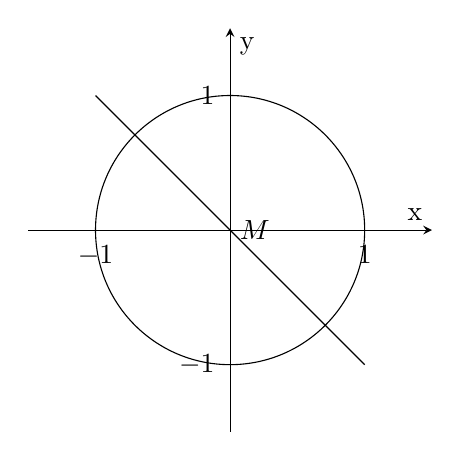
\begin{tikzpicture}
            \begin{axis}[xlabel={x}, ylabel={y}, xmin=-1.5, xmax=1.5, ymin=-1.5, ymax=1.5, axis lines = center, width=5cm, height=5cm, scale=1.5]
                \draw[black] (0, 0) circle [radius = 1] node[right] {$M$};
                \draw[domain = -1:1] plot(\x, -\x);
            \end{axis}
        \end{tikzpicture}
    \end{center}
\end{figure}

Пусть $M$ -- множество, которое задаётся ограничениями $g_i$. Разбор случаев (при помощи метода множителей Лагранжа):
\begin{enumerate}
    \item Кандидатов в точки экстремума внутри M:
        \[\left\{\begin{aligned}
            f^{'}_x = 0 \\
            f^{'}_y = 0 \\
            g_1 < 0 \\
            g_2 < 0
        \end{aligned}\right.\]
    \item Кандидаты на дуге окружности:
        \[\left\{\begin{aligned}
            f^{'}_x - \lambda_1 (g_1)^{'}_x = 0 \\
            f^{'}_y - \lambda_1 (g_2)^{'}_y = 0 \\
            g_1 = 0 \\
            g_2 < 0
        \end{aligned}\right.\]
    \item Кандидаты на отрезке внутри круга:
        \[\left\{\begin{aligned}
            f^{'}_x - \lambda_2 (g_2)^{'}_x = 0 \\
            f^{'}_y - \lambda_2 (g_2)^{'}_y = 0 \\
            g_2 = 0 \\
            g_1 < 0
        \end{aligned}\right.\]
    \item Кандидаты на пересечении окружности и прямой:
        \[\left\{\begin{aligned}
            f^{'}_x - \lambda_1 (g_1)^{'}_x - \lambda_2 (g_2)^{'}_x = 0 \\
            f^{'}_y - \lambda_1 (g_1)^{'}_y - \lambda_2 (g_2)^{'}_y = 0 \\
            g_1 = 0 \\
            g_2 = 0
        \end{aligned}\right.\]
\end{enumerate}
Далее во всех полученных кандидатах вычисляем целевую функцию.

\begin{theorem}{\textbf{Каруша-Куна-Таккера (простая версия для задачи с ограничениями типа неравенств).}}
Допустим, что $x^{(0)}$ -- решение задачи
$\begin{cases}
    f(x) \to extr \\
    g_i(x) \leqslant 0, i = 1, ..., m
\end{cases}$\\
Пусть $L(x, \lambda) = f(x) - \sum\limits_{i = 1}^{m} \lambda_i g_i(x)$ -- функция Лагранжа. Тогда в точке $x^{(0)}$ выполнено:
\[\left\{\begin{aligned}
    L^{'}_{x_j} &= 0, j = 1, ..., n\\
    g_i(x) &\leqslant 0, i = 1, ..., m\\
    \lambda_i g_i(x) &= 0, i = 1, ..., m \text{ -- условия дополняющей нежёсткости}
\end{aligned}\right.\]
\end{theorem}

\begin{remark}
В чём смысл условий дополняющей нежёсткости?\\
Если $\lambda_i > 0$, то соответствующее ограничение $g_i(x) \leqslant 0$ в решении задачи выполняется как равенство $g_i(x) = 0$ (т.е. это ограничение <<активно>>).\\
Если же $g_i(x) < 0$, то соответствующий множитель Лагранжа $\lambda_i$ должен быть равен нулю, и это ограничение не участвует в функции Лагранжа.
\end{remark}
\ProvidesFile{Q24.tex}[Билет 24]

\section{Билет 24. Дайте определение криволинейного интеграла 1-го рода и объясните, как такие интегралы вычисляются.}
Пусть $U \subset \mathbb{R}^n$ и $f: U \to \mathbb{R}$ -- непрерывная функция, $\gamma \subset U$ -- кривая
и $\gamma = \{x_j = \varphi_j(t) |\, j = 1, ..., n, \, t \in [a, b]\}$.
Пусть $(\tau, c)$ -- размеченное разбиение отрезка $[a, b]$, т.е. $\tau = (a = t_0 < t_1 < ... < t_m = b), c_i \in [t_{i - 1}, t_i]$.
\begin{definition}
    $|\tau| = \max\limits_{i}(t_i - t_{i - 1})$ -- диаметр разбиения $\tau$.
\end{definition}

\begin{remark}
    Более общее определение: $|\tau| = \max\limits_{i}(d_2(\varphi[t_i], \varphi[t_{i - 1}])$, где $d_2$ -- евклидова метрика.
\end{remark}

\begin{definition}
    Определим интегральную сумму (1-го рода) по кривой $\gamma$:
    \[
        S_{\tau, f, \gamma}^{I} = \sum_{i = 1}^{m} f\left[\varphi(c_i)\right] \Delta l_i
    \]
    \[
        \Delta l_i = d_2(\varphi(t_i), \, \varphi(t_{i - 1})) = \sqrt{\sum_{j = 1}^{n} (\varphi_j(t_i) - \varphi_j(t_{i - 1}))^2}
    \]
\end{definition}

\begin{definition}
    Предел $\lim\limits_{|\tau| \to 0} S_{\tau, f, \gamma}^{I} = \int\limits_{\gamma} f(x_1, ..., x_n)dl$ называется
    криволинейным интегралом 1-го рода от функции $f$ по кривой $\gamma$.
\end{definition}

\begin{remark}
    $\int\limits_{\gamma} f(x_1, ..., x_n)dl$ не зависит от параметризации кривой $\gamma$.
\end{remark}

\begin{remark}
    $dl$ называется элементом длины кривой. По теореме Пифагора:
    \[
        dl = \sqrt{(dx_1)^2 + ... + (dx_n)^2} = \left[x_j = \varphi_j(t)\right] =
        \sqrt{(\varphi_1^{'}(t)dt)^2 + ... + (\varphi_n^{'}(t)dt)^2} =
        \sqrt{\varphi_1^{'}(t)^2 + ... + \varphi_n^{'}(t)^2}dt
    \]
\end{remark}

\begin{statement}
    Пусть $\gamma$ задана параметрически: $x_j = \varphi_j(t), t \in [a, b]$ и $\varphi_j \in C^{1}([a, b])$. Тогда:
    \[
        \int\limits_{\gamma} f(x_1, ..., x_n)dl =
        \int\limits_{a}^{b} f[\varphi_1(t), ..., \varphi_n(t)]\sqrt{\varphi_1^{'}(t)^2 + ... + \varphi_n^{'}(t)^2}dt
    \]
\end{statement}

\textbf{Пример.}
\[
    \int\limits_{\gamma}1dl = \int\limits_a^b \sqrt{\sum_i (\varphi_i^{'})^2}dt \text{ -- длина кривой.}
\]

\ProvidesFile{Q25.tex}[Билет 25]

\section{Дайте определение криволинейного интеграла 2-го рода и объясните, как такие интегралы вычисляются.}
Пусть $U \subset \mathbb{R}^n$ и $f: U \to \mathbb{R}$ -- непрерывная функция, $\gamma \subset U$ -- кривая
и $\gamma = \{x_j = \varphi_j(t) |\, j = 1, ..., n, \, t \in [a, b]\}$.
Пусть $(\tau, c)$ -- размеченное разбиение отрезка $[a, b]$, т.е. $\tau = (a = t_0 < t_1 < ... < t_m = b), c_i \in [t_{i - 1}, t_i]$.

\textit{Мотивация.} Хотим определить $\int\limits_{\gamma} f(x_1, ..., x_n)dx_1$.

\begin{definition}
    Определим интегральную сумму (2-го рода) по кривой $\gamma$:
    \[
        S_{\tau, f, \gamma}^{II, \, x_1} = \sum_{i = 1}^{m} f\left[\varphi(c_i)\right] \Delta x_1
    \]
    \[
        \Delta x_1 = \varphi_1(t_i) - \varphi_1(t_{i - 1})
    \]
\end{definition}

\begin{definition}
    Предел $\lim\limits_{|\tau| \to 0} S_{\tau, f, \gamma}^{II} = \int\limits_{\gamma} f(x_1, ..., x_n)dx_1$ называется
    криволинейным интегралом 2-го рода от функции $f$ по кривой $\gamma$ по переменной $x_1$.
\end{definition}

\begin{remark}
    $\int\limits_{\gamma} f(x_1, ..., x_n)dx_1$  <<почти>> (т.е. с точностью до знака) не зависит от параметризации кривой $\gamma$.
\end{remark}

\begin{remark}
    $dx_1 = d\varphi_1(t) = \varphi_1^{'}(t)dt$
\end{remark}

\begin{statement}
    Пусть $\gamma$ задана параметрически: $x_j = \varphi_j(t), t \in [a, b]$ и $\varphi_j \in C^{1}([a, b])$. Тогда:
    \[
        \int\limits_{\gamma} f(x_1, ..., x_n)dx_1 =
        \int\limits_{a}^{b} f[\varphi_1(t), ..., \varphi_n(t)] \varphi_1^{'}(t)dt
    \]
    Аналогично определяются интегралы по любой другой координате.
\end{statement}

\textbf{Пример.}
\[
    \int\limits_{\gamma}1dx_1 = \int\limits_a^b \varphi_1^{'}(t)dt = \int\limits_a^b d(\varphi_1(t)) = \varphi_1(b) - \varphi_1(a)
    \text{ -- полное изменение первой координаты при движении по кривой.}
\]

\begin{remark}
    Более общо, можно брать интегралы от выражений вида $P_1(x_1, ..., x_n)dx_1 + P_2(x_1, ..., x_n)dx_2 + ... + P_n(x_1, ..., x_n)dx_n = \omega$:
    \[
        \int\limits_{\gamma} \omega :=
        \int\limits_{\gamma} P_1dx_1 + ... + \int\limits_{\gamma} P_ndx_n =
        \int\limits_{a}^{b} \left[P_1(\varphi(t)) P_1^{'} + P_n(\varphi(t)) P_n^{'}\right]dt
    \]
\end{remark}

\begin{definition}
    Выражения вида $P_1(x_1, ..., x_n)dx_1 + P_2(x_1, ..., x_n)dx_2 + ... + P_n(x_1, ..., x_n)dx_n$ называются дифференциальными 1-формами
    (или формами ранга 1).
\end{definition}

\begin{definition}
    Выражения вида $\int\limits_{\gamma} \omega$ называются интегралами 2-го рода от 1-формы $\omega$ по кривой $\gamma$.
\end{definition}

\ProvidesFile{Q26.tex}[Билет 26]

\section{Билет 26. Объясните, почему криволинейный интеграл 1-го рода не зависит от ориентации кривой, а криволинейный
интеграл 2-го рода -- зависит.}
\begin{definition}
    Предел $\lim\limits_{|\tau| \to 0} S_{\tau, f, \gamma}^{I} = \int\limits_{\gamma} f(x_1, ..., x_n)dl$ называется
    криволинейным интегралом 1-го рода от функции $f$ по кривой $\gamma$.
\end{definition}

\begin{remark}
    $dl$ называется элементом длины кривой. По теореме Пифагора:
    \[
        dl = \sqrt{(dx_1)^2 + ... + (dx_n)^2} = \left[x_j = \varphi_j(t)\right] =
        \sqrt{(\varphi_1^{'}(t)dt)^2 + ... + (\varphi_n^{'}(t)dt)^2} =
        \sqrt{\varphi_1^{'}(t)^2 + ... + \varphi_n^{'}(t)^2}dt
    \]
\end{remark}

\begin{definition}
    Предел $\lim\limits_{|\tau| \to 0} S_{\tau, f, \gamma}^{II} = \int\limits_{\gamma} f(x_1, ..., x_n)dx_1$ называется
    криволинейным интегралом 2-го рода от функции $f$ по кривой $\gamma$ по переменной $x_1$.
\end{definition}

\begin{remark}
    $dx_1 = d\varphi_1(t) = \varphi_1^{'}(t)dt$
\end{remark}

При изменении направления обхода интеграл 2-го рода меняет знак, а интеграл 1-го рода не меняет знак. Почему?
Заметим следующее: в интегралах 2-го рода стоят выражения $dx_1, ..., dx_n$, которые меняют знак при изменении направления обхода,
а элемент длины $dl = \sqrt{(dx_1)^2 + ... + (dx_n)^2}$ не зависит от знаков выражений $dx_1, ..., dx_n$.

\begin{remark} Подробнее про смену знака $dx_i$ (из билета 25).\\
    Определим интегральную сумму (2-го рода) по кривой $\gamma$:
    \[
        S_{\tau, f, \gamma}^{II, \, x_1} = \sum_{i = 1}^{m} f\left[\varphi(c_i)\right] \Delta x_1
    \]
    \[
        \Delta x_1 = \varphi_1(t_i) - \varphi_1(t_{i - 1})
    \]
    Видим, что $\Delta x_i$ в определении интегральной суммы зависит от порядка обхода сегментов разбиения.
\end{remark}
\ProvidesFile{Q27.tex}[Билет 27]

\section{Билет 27. Сформулируйте формулу Грина и докажите её для области $\Omega \subset \mathbb{R}^2$ вида $\Omega = [a, b] \times [c, d]$ (прямоугольник).}

\begin{theorem}{Формула Грина.}\\
    Пусть $U \subset \mathbb{R}^2$ -- связное подмножество, ограниченное кусочно-гладкой кривой $\partial U = \Gamma$ (граница множества $U$).
    Зафиксируем ориентацию на $\Gamma$, обход вдоль которой всегда оставляет область $U$ слева. Пусть функции $P(x, y), Q(x, y)$ дифференцируемы
    в некоторой окрестности $U$. Тогда верно следующее:
    \begin{enumerate}
        \item \[ \int\limits_{\Gamma} P(x, y)dx = \iint\limits_{U} -\frac{\partial P}{\partial y}dxdy \]
        \item \[ \int\limits_{\Gamma} Q(x, y)dy = \iint\limits_{U} \frac{\partial Q}{\partial x}dxdy \]
        \item \[ \int\limits_{\Gamma} Pdx + Qdy =
                \iint\limits_{U} \left(\frac{\partial Q}{\partial x} - \frac{\partial P}{\partial y}\right)dxdy \text{ -- формула Грина}\]
    \end{enumerate}
\end{theorem}

\begin{proof}
    План:
    \begin{enumerate}
        \item Докажем формулу 1.
        \item Формула 2 доказывается аналогично при помощи замены $x \leftrightarrow y$.
        \item Формула 3 суть сумма формул 1 и 2.
    \end{enumerate}
    Будем предполагать, что $U = \left\{ (x, y) \, | a \leqslant x \leqslant b, c \leqslant y \leqslant d \right\}$,
    т.е. $U$ -- прямоугольник.\\
    $\Gamma = \partial U = \Gamma_1 \cup \Gamma_2 \cup \Gamma_3 \cup \Gamma_4$, где $\Gamma_1, \Gamma_2$ -- горизонтальные отрезки ($y = c, y = d$),
    а $\Gamma_3, \Gamma_4$ -- вертикальные отрезки. Тогда:
    \[
        \int\limits_{\Gamma} Pdx =
        \int\limits_{\Gamma_1} Pdx + \int\limits_{\Gamma_2} Pdx + \int\limits_{\Gamma_3} Pdx + \int\limits_{\Gamma_4} Pdx
    \]
    Заметим, что $\int\limits_{\Gamma_3} Pdx + \int\limits_{\Gamma_4} Pdx = 0$,
    т.к. на вертикальных отрезках выполнено, что $x = const \Rightarrow dx = 0$.\\
    Параметризуем: $\Gamma_1 = \begin{cases} x = t\\ y = c\end{cases} t \in [a, b]$, $\Gamma_2 = \begin{cases} x = t\\ y = d\end{cases} t \in [b, a]$.
    Интегрируем по определению:
    \[
        \int\limits_{a}^{b} P(t, c)dt - \int\limits_{a}^{b} P(t, d)dt =
        \int\limits_{a}^{b} \left[P(t, c) - P(t, d) \right] dt = \star
    \]
    Заметим, что подынтегральное выражение равно (по формуле Ньютона-Лейбница):
    \[
        \int\limits_{d}^{c} \frac{\partial P}{\partial y}(t, s)ds =
        -\int\limits_{c}^{d} \frac{\partial P}{\partial y}(t, s)ds
    \]
    Подставим:
    \[
        \star = -\int\limits_a^b \left[\int\limits_{c}^{d} \frac{\partial P}{\partial y}(t, s)ds \right]dt = [\text{Переходим к кратному интегралу}] =
        -\iint\limits_{U} \frac{\partial P}{\partial y}dxdy
    \]
\end{proof}



\setcounter{section}{27}
	\section{Дайте определение элемента площади 2-мерной поверхности в $\mathbb{R}^3$ и поверхностного интеграла 1-го рода}

	Пусть имеется двумерная поверхность $\Omega \subseteq \mathbb{R}^3$ и у неё зафиксирована параметризация $\varphi:M \to \Omega, M \subseteq \mathbb{R}^2$. Будем обозначать координаты в $\mathbb{R}^3$ как $(x, y, z)$, а в $\mathbb{R}^2$ ---~ как $(u, v)$. Неформально говоря, элементом площади в точке поверхности называется площадь бесконечно малого параллелограмма со сторонами, направленными параллельно касательным векторам в этой точке. Можно провести аналогию с одномерными интегралами, где мы приближаем функцию с помощью ломаной с маленькими звеньями, и сказать, что мы приближаем поверхность маленькими чешуйками в форме параллелограммов. Запишем теперь формулу для элемента площади в точке $(u, v)$
	
	\[ \diff S = S(P(\varphi'_u(u, v), \varphi'_v(u, v))) \diff u \diff v; \]

	Здесь $\varphi'_u, \varphi'_v$ --- трёхмерные векторы (так как $\varphi$ имеет три координаты), именно они являются касательными в данной точке; $P$ ---~ параллелограмм, натянутый на векторы; $S$ ---~ площадь. Из линейной алгебры мы знаем, что площадь параллелограмма можно считать как корень из определителя матрицы Грама его сторон. Это даёт нам новую формулу для элемента площади.

	\[ \diff S = \sqrt{EG - F^2}\diff u \diff v; \]
	
	Здесь $E = \langle \varphi'_u, \varphi'_u \rangle = \| \varphi'_u \|^2, G = \langle \varphi'_v, \varphi'_v \rangle = \| \varphi'_v \|^2, F = \langle \varphi'_u, \varphi'_v \rangle$. 

	Теперь мы можем естественным образом определить поверхностный интеграл 1-го рода от функции $f:\mathbb{R}^3 \to \mathbb{R}$ по $\Omega$.

	\[ \iint\limits_\Omega f(x, y, z) \diff S := \iint\limits_M f(\varphi(u, v)) \sqrt{E(u, v)G(u, v) - F^2(u, v)} \diff u \diff v; \]

	Здесь мы опираемся на параметризацию при определении интеграла. Можно проверить, что при смене параметризации значение интеграла 1-го рода не изменится. 

	\section{Дайте определение элемента $k$-мерного объёма $k$-мерного многообразия в $\mathbb{R}^n$ и интеграла 1-го рода по $k$-мерному многообразию}

	Пусть имеется $k$-мерное многообразие $\Omega \subseteq \mathbb{R}^n$ и у него зафиксирована параметризация $\varphi: M \to \Omega, M \subseteq \mathbb{R}^k$. Будем обозаначать координаты в $\mathbb{R}^n$ как $x = (x_1, \ldots, x_n)$, а в $\mathbb{R}^k$ ---~ как $t = (t_1, \ldots, t_k)$. Аналогично предыдущему билету, определим элемент $k$-мерного объёма в точке $t$.

	\[ \diff \! \mathit{Vol}_k = S(P(\varphi'_{t_1}(t), \ldots, \varphi'_{t_k}(t))) \diff t_1 \ldots \diff t_k; \]

	Запишем теперь формулу для интеграла 1-го рода от функции $f:\mathbb{R}^n \to \mathbb{R}$ по $\Omega$.

	\[ \int\limits_\Omega f(x) \diff \! \mathit{Vol}_k := \int\limits_M f(\varphi(t))S(P(\varphi'_{t_1}(t), \ldots, \varphi'_{t_k}(t))) \diff t_1 \ldots \diff t_k;  \]

	Опять же, можно проверить, что интеграл 1-го рода не зависит от параметризации.

	\section{Объясните, что такое грассманово умножение, грассмановы переменные, грассмановы мономы}

	Пусть у нас имеется набор символов $a_1, \ldots, a_n$ ---~ грассмановых переменных и мы умеем брать их линейные комбинации. То есть, например, у нас есть отдельные элементы $a_2 - a_1, 0, -5a_3$ и т. п. Теперь мы хотим ввести новую операцию ---~ научиться умножать наши элементы друг на друга. Наше умножение будет обозначаться символом $\land$ и называться грассмановым умножением. Умножение будет удовлетворять всем стандартным требованиям, кроме коммутативности, которую мы заменим на более странное свойство 4:

	\begin{enumerate}
		\item $(x \land y) \land z = x \land (y \land z);$
		\item $(x + y) \land z = x \land z + y \land z;$
		\item $z \land (x + y) = z \land x + z \land y;$
		\item $a_i \land a_j = -a_j \land a_i;$
	\end{enumerate}

	Обратите внимание, пункты 1-3 относятся к любым элементам, а пункт 4 только к исходным $a_1, \ldots, a_n$. Простые следствия из свойств: $0 \land x = 0, a_i \land a_i = 0$. Для примера посчитаем <<квадрат>> элемента $a_1 \land a_2 + a_3$.
	
	\[ (a_1 \land a_2 + a_3) \land (a_1 \land a_2 + a_3) = a_1 \land a_2 \land (a_1 \land a_2 + a_3) + a_3 \land (a_1 \land a_2 + a_3) = 0 + a_1 \land a_2 \land a_3 + a_3 \land a_1 \land a_2 + 0 = \] \[ = a_1 \land a_2 \land a_3  - a_1 \land a_3 \land a_2 = a_1 \land a_2 \land a_3 + a_1 \land a_2 \land a_3 = 2a_1 \land a_2 \land a_3;\]

	\begin{definition}
		\textit{Грассмановым мономом} степени $k$ называется элемент вида $\alpha a_{i_1} \land \ldots \land a_{i_k}$, где $ i_1, \ldots i_k \in \{0, \ldots, n \}$, $\alpha$ ---~ некоторый коэффициент.
	\end{definition}

	Заметим, что если среди $i_1, \ldots i_k$ есть повторения, то моном равен нулю. Переменные в грассмановом мономе можно отсортировать, возможно, поменяв при этом знак. Точнее, при сортировке моном домножится на -1 в степени равной числу инверсий, то есть на знак перестановки.

	\section{Объясните, что такое дифференциальная форма ранга $k$, и как вычисляется интеграл (2-го рода) от $k$-формы $\omega$ по $k$-мерному многообразию $\Omega \subseteq \mathbb{R}^n$. Запишите вычислительную формулу для поверхностного интеграла 2-го рода}

	\begin{definition}
		\textit{Дифференциальной формой} ранга $k$ (или дифференциальной $k$-формой) на $M \subseteq \mathbb{R}^n$ называется выражение вида $\sum\limits_{\{i_1, \ldots, i_k\} \subseteq \{1, \ldots, n\}} f_{i_1 \ldots i_k}(x)\diff x_{i_1} \land \ldots \land \diff x_{i_k}$, где $f_{i_1\ldots i_k}$ ---~ некоторые дифференцируемые\footnote{Часто ограничиваются гладкими функциями.} функции $f_{i_1\ldots i_k}:M \to \mathbb{R}$.
	\end{definition}

	Если вам очень понравился предыдущий билет, можно сказать, что это сумма грассмановых мономов степени $k$ от переменных $\diff x_1, \ldots \diff x_n$ с дифференцируемыми функциями в качестве коэффициентов. Можно считать, что среди чисел $i_1, \ldots, i_k$ нет повторений, так как мономы с повторениями всё равно зануляются.

	Пусть имеются $k$-мерное многообразие $\Omega \subseteq \mathbb{R}^n$ с параметризацией $\varphi: M \to \Omega, M \subseteq \mathbb{R}^k$ и дифференциальная $k$-форма $\omega = \sum\limits_{\{i_1, \ldots, i_k\} \subseteq \{1, \ldots, n\}} f_{i_1 \ldots i_k}(x)\diff x_{i_1} \land \ldots \land \diff x_{i_k}$ на $\Omega$. Определим интеграл (2-го рода) $\omega$ по $\Omega$.

	\[ \int\limits_\Omega \omega := \int\limits_M \sum_{\{i_1, \ldots, i_k\} \subseteq \{1, \ldots, n\}} f_{i_1 \ldots i_k} (\varphi(t)) \diff \varphi_{i_1} \land \ldots \land \diff \varphi_{i_k}; \]

	Поясним, что творится в этой формуле. Во-первых, $\varphi_i : M \to \mathbb{R}$ ---~ это функция, соответствующая $i$-й координате $\varphi$. Во-вторых, $\diff \varphi_i$ ---~ это привычный дифференциал функции нескольких переменных, но теперь мы говорим, что это линейная комбинация грассмановых переменных $\diff t_1, \ldots, \diff t_k$. Когда мы грассманово перемножим эти дифференциалы, у нас останется выражение вида $f(t) \diff t_1 \land \ldots  \land \diff t_k$. Это так, ведь в любом слагаемом результата будут перемножаться $k$ переменных, одинаковые занулятся, останутся только слагаемые с различными, возможно, не в том порядке. Но мы можем привести порядок к правильному. После этих преобразований мы считаем интеграл как обычный кратный интеграл.
\[\int\limits_M f \diff t_1 \land \ldots \land \diff t_k = \int\limits_M f \diff t_1 \ldots \diff t_k;  \]  

	Для случая $k = 2$ это всё можно записать в следующую формулу.

	\[\iint\limits_\Omega P\diff y \land \diff z + Q \diff z \land \diff x + R \diff x \land \diff y = \iint\limits_M \begin{vmatrix} P & Q & R \\ \frac{\partial \varphi_1}{\partial u} & \frac{\partial \varphi_2}{\partial u} & \frac{\partial \varphi_3}{\partial u} \\ \frac{\partial \varphi_1}{\partial v} & \frac{\partial \varphi_2}{\partial v} & \frac{\partial \varphi_3}{\partial v} \end{vmatrix} \diff u \diff v;\]

	Обратите внимание, при $Q$ стоит $\diff z \land \diff x$, а не $\diff x \land \diff z$. 

	\section{Что такое ориентация $k$-мерного многообразия? Как изменится интеграл 2-го рода от дифференциальной формы при смене ориентации многообразия (б. д.)?}

	Пусть $\Omega \subseteq \mathbb{R}^n$ ---~ $k$-мерное связное\footnote{Напомним, многообразие называется гладким, если любые две его точки можно соединить проходяще по нему непрерывной кривой.} многообразие, и у него имеются две параметризации $\varphi: M \to \Omega, \psi: N \to \Omega; M, N \subseteq \mathbb{R}^k$. Предположим, что функция замены координат $c = \varphi^{-1} \circ \psi$ биективна и непрерывно дифференцируема.

	\[ \begin{tikzcd}
		M \arrow[swap]{rd}{\varphi} &  &\arrow[swap]{ll}{c} N \arrow{ld}{\psi} \\
		& \Omega
	\end{tikzcd} \]

	Посмотрим на якобиан $J(c)$. Если бы где-то он был равен нулю, в окрестности этой точки $c$ была бы необратима. Значит он не равен нулю нигде. Поскольку $J(c)$ непрерывен и $\Omega$ связно, из этого следует, что он имеет постоянный знак. Тогда если он положителен, будем говорить, что $\varphi$ и $\psi$ задают одну и ту же ориентацию, а если отрицателен ---~ то разные. Таким образом мы определяем ориентацию как отношение эквивалентности с двумя классами на параметризациях многообразия.

	Ориентация задаёт ориентацию на любом касательном пространстве $T_{x}\Omega$ как на векторном пространстве. Если мы назвали ориентацию некоторой параметризации положительной, то назовём положительным базис $T_x \Omega$, полученный из её производных.

	При смене параметризации на имеющую противоположную ориентацию интеграл 2-го рода меняет знак. 

	\section{Дайте определение согласованных ориентаций многообразия и его границы. Дайте определение дифференциала от $k$-формы. Запишите общую формулу Стокса.}
	Будем обозначать границу многообразия $\Omega$ как $\partial \Omega$. Заметим, что если у $k$-мерного многообразия есть граница, то она имеет размерность $k - 1$.

	\begin{definition}
		Будем говорить, что ориентации $\Omega$ и $\partial \Omega$ согласованы, если для любой точки $x \in \partial \Omega$ для любого положительного базиса $v_1, \ldots v_{k - 1}$ в $T_x \partial \Omega$, базис $v_1, \ldots, v_{k - 1}, \vec{n}$ положителен в $T_x \Omega$, где $\vec{n}$ ---~ это вектор в $T_x \Omega$, перпендикулярный $T_x \partial \Omega$ и смотрящий наружу\footnote{Это можно формализовать, например, как отрицательное скалярное произведение с любым вектором, соединяющим $x$ и точку из окрестности $x$ из $\Omega$. Но лектор это никак не формализовал.} $\Omega$.
	\end{definition}

	Мы привыкли, что дифференциал суммы равен сумме дифференциалов. Поэтому для определения дифференциала от дифференциальной формы достаточно определить дифференциал от грассманова монома.

	\[ \diff(f \diff x_{i_1} \land \ldots \land \diff x_{i_k}) := \diff f \land \diff x_{i_1} \land \ldots \land \diff x_{i_k}; \]

	\begin{remark}
		Дифференциал $k$-формы является $(k + 1)$-формой.
	\end{remark}

	Для примера посчитаем дифференциал от дифференциала некоторой функции $f:\mathbb{R}^n \to \mathbb{R}$.

	\[\diff (\diff f) = \diff \left(\sum_{i = 1}^n \frac{\partial f}{\partial x_i}\diff x_i \right) = \sum_{i = 1}^n \sum_{j = 1}^n \frac{\partial^2 f}{\partial x_i \partial x_j} \diff x_j \land \diff x_i; \]

	При этом слагаемые вида $\frac{\partial^2 f}{\partial x_i \partial x_i} \diff x_i \land \diff x_i$ сразу зануляются, а слагаемые вида $\frac{\partial^2 f}{\partial x_i \partial x_j} \diff x_j \land \diff x_i$ сократятся с $\frac{\partial^2 f}{\partial x_j \partial x_i} \diff x_i \land \diff x_j$. Значит $\diff(\diff f) = 0$.

	Пусть теперь $\Omega \subseteq \mathbb{R}^n$ ---~ $k$-мерное многообразие с согласованными ориентациями на самом многообразии и на границе, а $\omega$ ---~ дифференциальная $(k - 1)$-форма на $\Omega$. Тогда верна (общая) формула Стокса:

	\[ \int\limits_{\partial \Omega} \omega = \int\limits_\Omega \diff \omega; \] 

	\section{Выведите из общей формулы Стокса частные случаи: формулу Ньютона-Лейбница, формулу Грина, формулу Гаусса-Остроградского.}

	\subsection*{Формула Ньютона-Лейбница, $n = k = 1$}

	Пусть наше многообразие это отрезок на прямой $[a; b]$. Его границей будет множество из двух точек $\{a, b\}$. Заметим, что точка ---~ это нульмерное многообразие и по нему можно интегрировать 0-формы (то есть просто функции). При чём этот интеграл будет с точностью до знака (знак как всегда определяется ориентацией) равен значению функции в точке. Если на отрезке мы берём стандартную ориентацию <<слева направо>>, то для границы это будет означать взятие $b$ с плюсом и $a$ с минусом. Итак, формула Стокса принимает следующий вид:
	
	\[F(b) - F(a) = \int\limits_a^b \diff F; \]
	
	Перепишем в более привычную запись.

	\[\int\limits_a^b F'(x) \diff x = F(b) - F(a); \]

	\subsection*{Формула Грина, $n = k = 2$}

	Дифференциальная 1-форма в $\mathbb{R}^2$ имеет вид $P\diff x + Q \diff y$. Посчитаем её дифференциал

	\[\diff (P \diff x + Q \diff y) = \left(\frac{\partial P}{\partial x}\diff x + \frac{\partial P}{\partial y}\diff y \right) \land \diff x +\left(\frac{\partial Q}{\partial x}\diff x + \frac{\partial Q}{\partial y}\diff y \right) \land \diff y = \frac{\partial P}{\partial y} \diff y \land \diff x + \frac{\partial Q}{\partial x} \diff x \land \diff y = \] \[ = \left(\frac{\partial Q}{\partial x} - \frac{\partial P}{\partial y}\right) \diff x \land \diff y;  \]

	Формула Стокса принимает следующий вид:

	\[\int\limits_{\partial U} P\diff x + Q\diff y = \iint\limits_{U} \left(\frac{\partial Q}{\partial x} - \frac{\partial P}{\partial y}\right)\diff x \diff y; \]

	Здесь условие согласованности ориентации можно сформулировать как <<при обходе $\partial U$ по заданной параметризации $U$ всегда находится слева>>.

	\subsection*{Формула Гаусса-Остроградского, $n = k = 3$}

	Дифференциальная 2-форма в $\mathbb{R}^3$ имеет вид $P\diff y \land \diff x + Q \diff z \land \diff x + R \diff x \land \diff y$. Посчитаем её дифференциал.

	\[\diff (P\diff y \land \diff z + Q \diff z \land \diff x + R \diff x \land \diff y) = \frac{\partial P}{\partial x} \diff x \land \diff y \land \diff z + \frac{\partial Q}{\partial y}\diff y \land \diff z \land \diff x + \frac{\partial R}{\partial z} \diff z \land \diff x \land \diff y  = \] \[ =\left( \frac{\partial P}{\partial x} + \frac{\partial Q}{\partial y} + \frac{\partial R}{\partial z} \right) \diff x \land \diff y \land \diff z; \]

	Формула Стокса принимает следующий вид:

	\[\iint\limits_{\partial V} P\diff y \land \diff x + Q \diff z \land \diff x + R \diff x \land \diff y = \iiint\limits_{V}\left( \frac{\partial P}{\partial x} + \frac{\partial Q}{\partial y} + \frac{\partial R}{\partial z} \right) \diff x\diff y\diff z; \]
\end{document}